\chapter{系统功能的具体实现}
基于SDN的云平台多租户虚拟网络定制化研究的实现,需要完成系统的搭建,实现系统各模块功能。系统架构中,网路虚拟化模块,需要完成虚拟网络的创建、删除工作;通信模块实现进程间的异步通信;控制器模块主要进行带宽、时延的测量工作,以及通过定制化流表的下发完成链路的选取;GUI模块主要实现拓扑信息、虚拟网络创建、测量数据展示的功能。各模块之间协同工作,实现基于SDN的云平台多租户虚拟网络的定制化。
\section{网络虚拟化模块}
\subsection{虚拟化和去虚拟化流程}
网络虚拟化模块,主要包含虚拟化和去虚拟化两个方面,如第三章图\ref{fig:virtual}所示。主要涉及到交换机的转换、OpenFlow字段转换(包括Cookie、Buffer\ ID, XID)、地址的虚拟化。其中对于交换机的转换,包括针对租户控制器发送的南向消息,进行去虚拟化,由VirtualSwitch映射成PhysicalSwitch;针对底层物理网络的北向消息,进行虚拟化操作,由PhysicalSwitch映射成VirtualSwitch。地址的虚拟化,是针对主机创建VirtualIP和PhysicalIP,以避免租户流量之间存在地址空间冲突,图\ref{fig:addr-vir}描述了地址虚拟化的具体过程。

\begin{figure}[!htb]
  \centering
  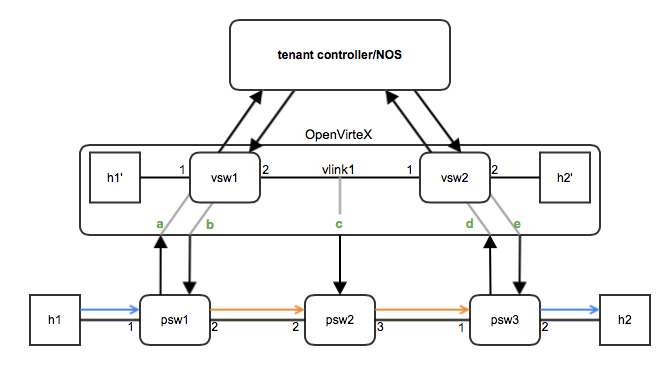
\includegraphics[width=0.7\textwidth]{logo/addr_virt}
  \caption{地址虚拟化过程}
  \label{fig:addr-vir}
\end{figure}

虚拟化流程如下:
\begin{enumerate}[a)]
\item PacketIn消息携带VirtualIP,未经修改直接发送给租户控制器
\item 相应的FlowMod匹配VirtualIP,执行的OFAction为将值修改为PhysicalIP。
\item 虚拟链路通过核心侧交换机psw2映射回两跳路径。
\item 目的地边缘的PacketIn与核心网络中的转换行为一致。
\item 虚拟化平台下发与PhysicalIP匹配的FlowMod消息。执行的OFAction为重写回VirtualIP。
\end{enumerate}

转换的过程主要对PacketIn、PacketOut和FlowMod消息的虚拟化与去虚拟化。针对PacketIn消息,由于该消息是来自南向物理交换机,所以消息的处理过程为虚拟化过程,具体的虚拟化过程如图\ref{fig:packetin}所示。首先判断该数据报是否来自边缘侧交换机,如果是,直接查看租户ID和虚拟交换机,如果不是,通过对数据域的匹配,获取租户的ID和虚拟交换机,进而检查该租户的控制器是否以建立连接,如果建立连接,直接将消息发送给租户控制器,否则丢弃。针对L3层的数据报,首先检查PhysicalIP的合理性,在合理的情况下,查看虚拟IP和交换机,并将数据包中的IP地址进行重写。

\begin{figure}[!htb]
  \centering
  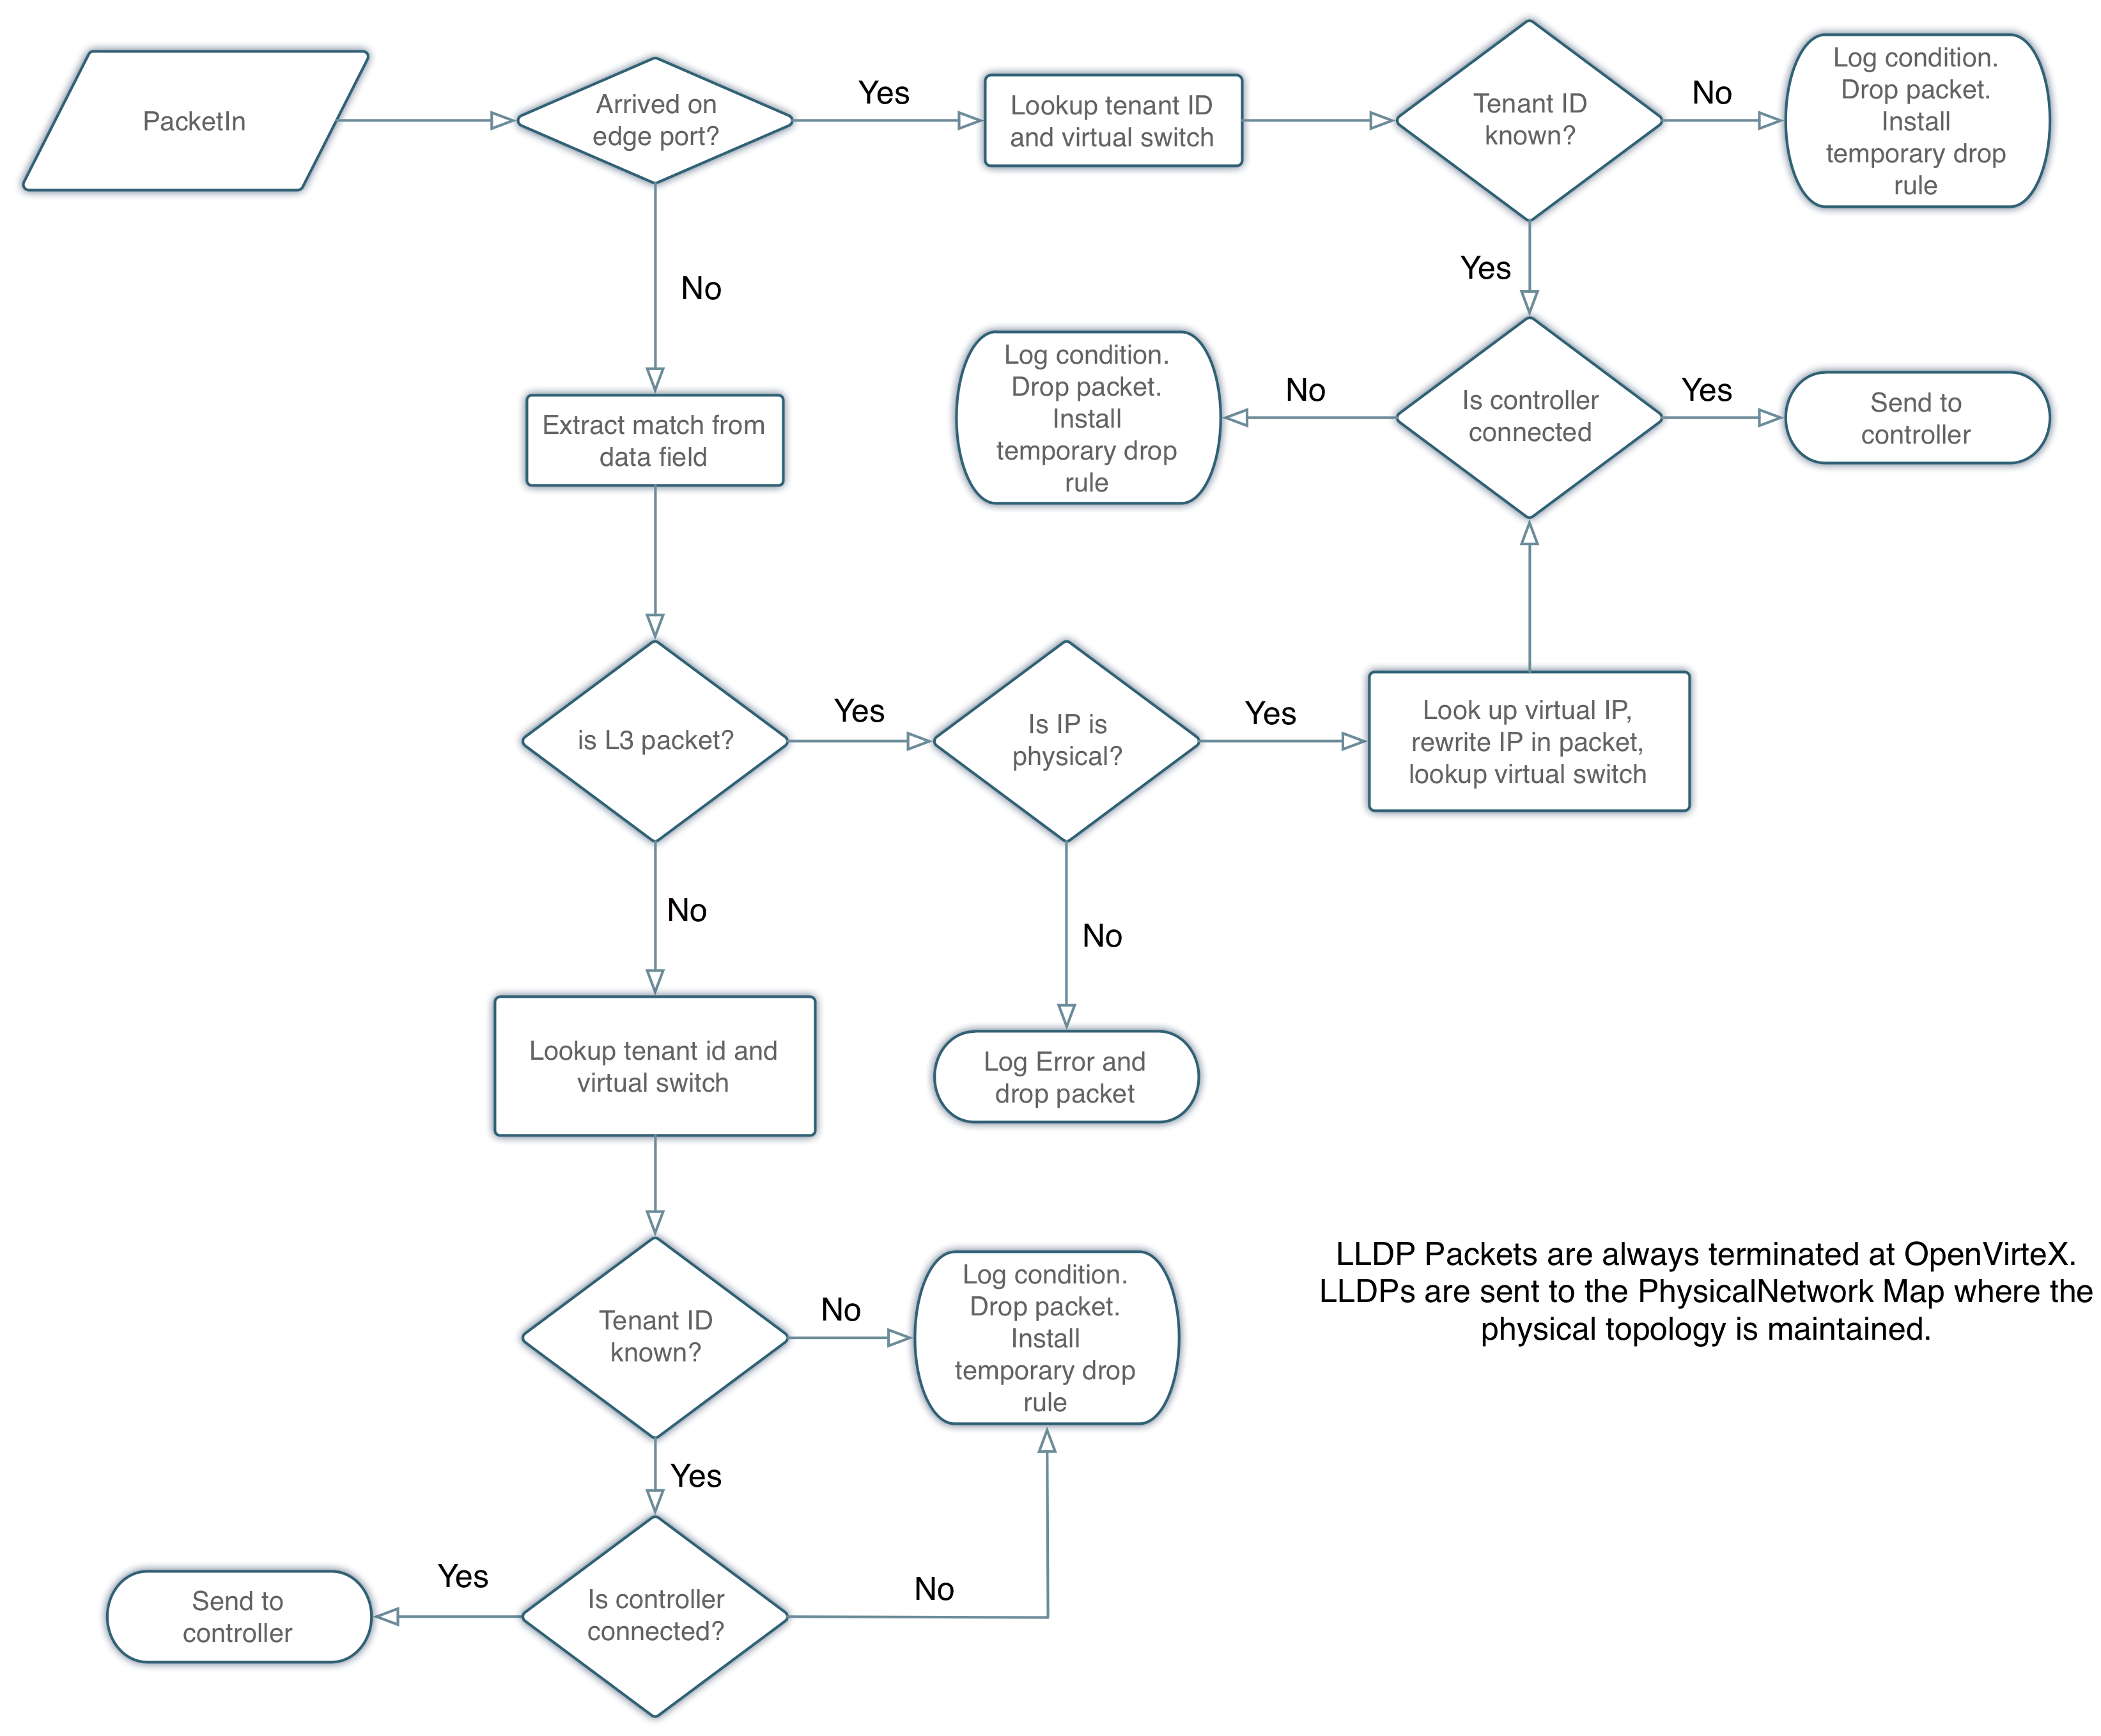
\includegraphics[width=0.7\textwidth]{logo/PacketIn}
  \caption{PacketIn虚拟化}
  \label{fig:packetin}
\end{figure}

针对PacketOut消息,由于该消息是由北向租户控制器下发给交换机,所以该消息的处理过程是去虚拟化过程,具体的去虚拟化过程如图\ref{fig:packetout}所示,首先检查bufferID的合理性,进而从data中提取匹配域,重写端口以及bufferID等信息,将action中的地址,修改为PhysicalIP。

\begin{figure}[!htb]
  \centering
  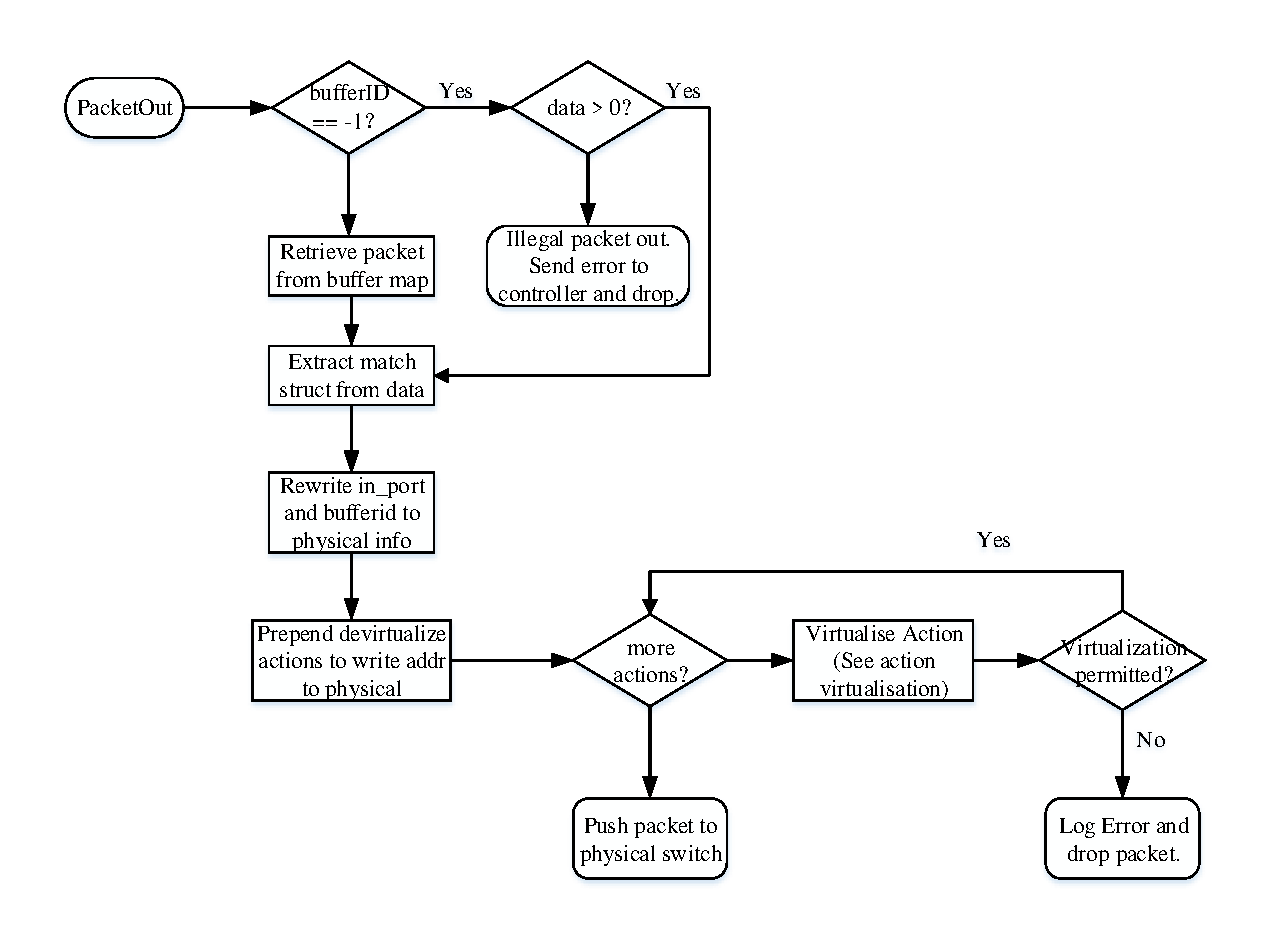
\includegraphics[width=0.7\textwidth]{logo/PacketOut}
  \caption{PacketOut去虚拟化}
  \label{fig:packetout}
\end{figure}

针对FlowMod消息,由于该消息是由北向租户控制器发送给交换机,因此,该过程也是一个去虚拟化的过程。首先需要判断该条流是来自入口交换机、出口交换机,还是核心交换机,针对不同的情况进行具体的操作。如果该消息来自出口交换机或者核心交换机,需要将匹配域重写为PhysicalIP,然后,依次将执行的动作重写为物理地址,然后将消息下发给物理交换机,具体如图\ref{fig:flowmod}所示。

\begin{figure}[!htb]
  \centering
  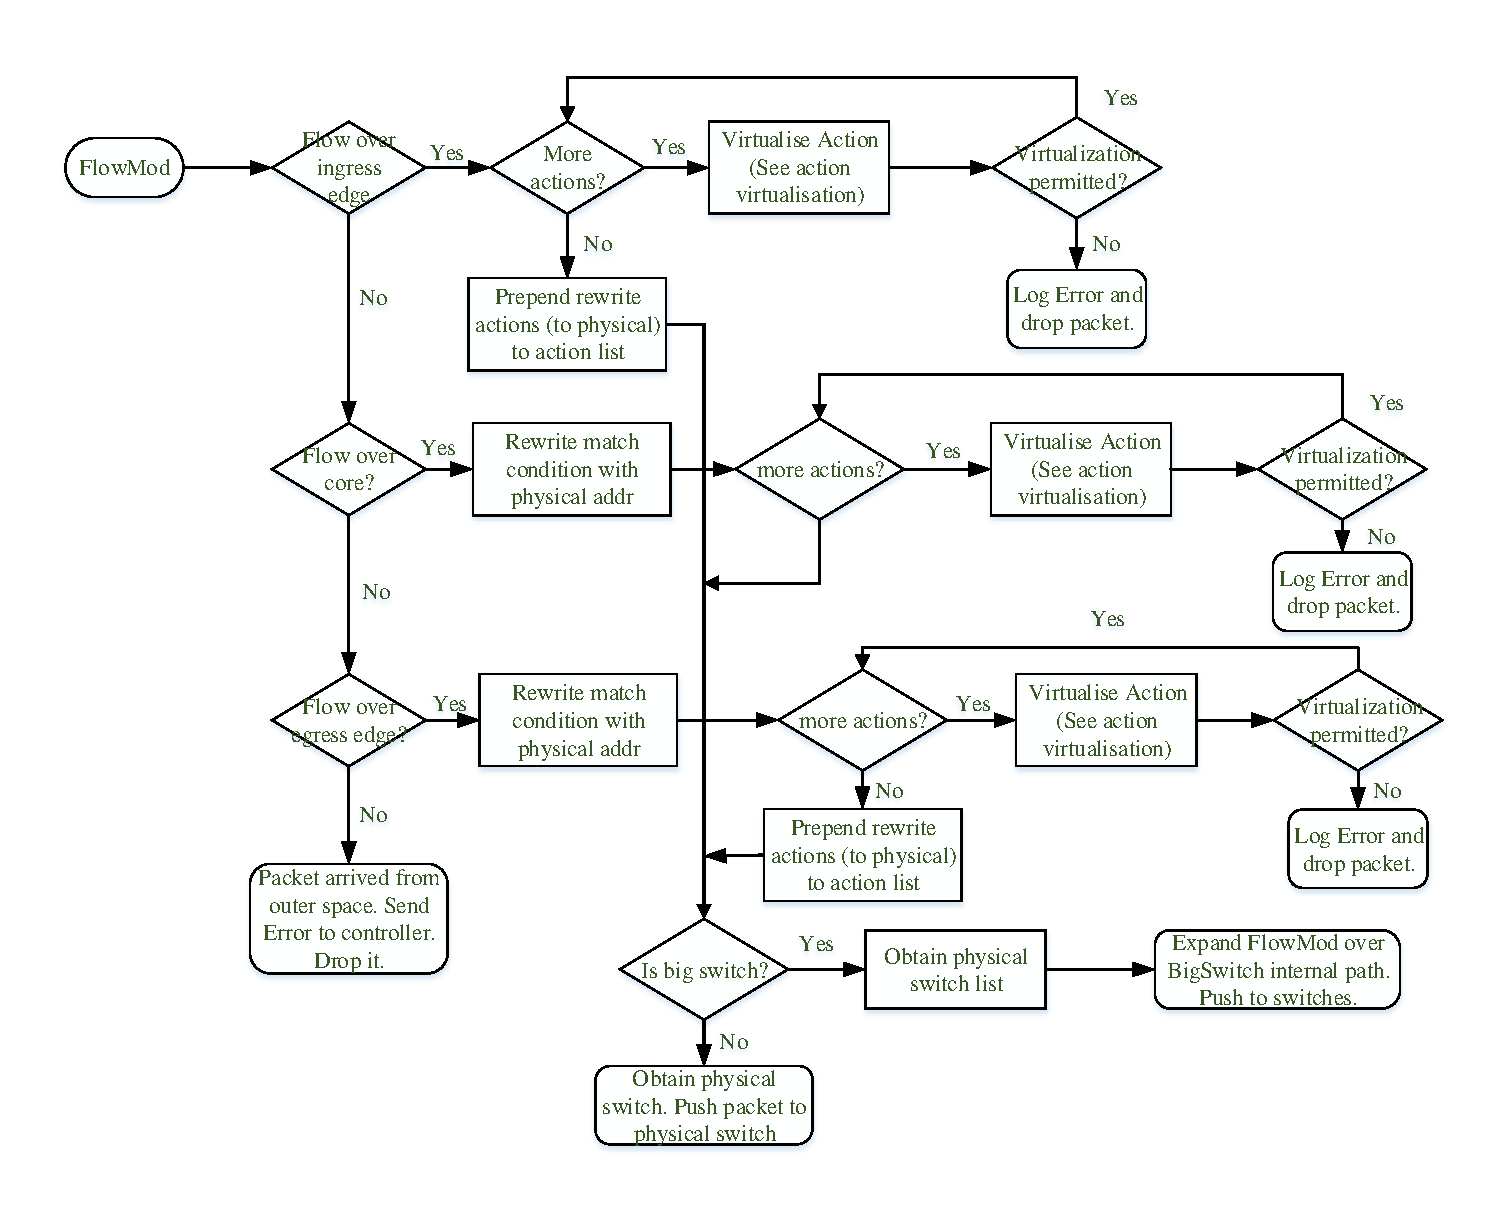
\includegraphics[width=0.7\textwidth]{logo/FlowMod}
  \caption{FlowMod虚拟化}
  \label{fig:flowmod}
\end{figure}
\subsection{虚拟网络创建}
针对虚拟网络的创建,本文为虚拟化平台封装了API接口\emph{createCustomNetwork},该接口的输入数据为Json格式的拓扑信息,具体信息格式如下图所示,由图中可以看出,主要由subnet,switches,hosts,ctrls,method,routing组成,subnet描述了虚拟网络的网络地址信息,不同的租户可以共用相同的网络地址;hosts和switches描述了底层网路的交换机和主机信息,虚拟网络映射到相应的物理组件上;ctrls描述了虚拟网路的控制器信息,创建的虚拟网络由该控制器进行集中管控;method为创建虚拟网络的方式,现有模式下有两种方式,其一是虚拟网络与物理网络的节点是一一对应的,其二是big\ switch的创建,即租户的单个虚拟交换机映射到底层的多个物理交换机,实现物理网络侧多对一的映射,本文虚拟网络的创建默认采用一一对应的映射模型;routing描述了虚拟网络的路由算法,现阶段网络虚拟化平台仅仅提供了spf路由算法。租户根据虚拟化平台管控的物理拓扑信息,选取出进行虚拟网络创建的主机和交换机,配置好虚拟网络的子网信息和控制器信息,按照规定的格式发送至虚拟化平台进行虚拟网络的创建。

\begin{python} 
topo = {
	'subnet':'type:str', #虚拟网络的网络地址/位数,例如'192.168.0.0/24'
	'switches':[
		{
			'dpid':'type:str'
		}
	], #物理交换机列表,列表中的每个交换机由dpid标识
	'hosts':[
		{
			'mac':'type:str',
			'port':'type:int',
			'dpid':'type:str'
		}
	], #物理主机列表,列表中每条主机信息为dict,存储主机的mac地址、连接物理交换机的dpid和port
	'ctrls':'type:str', #租户控制器信息,包括租户控制器所在IP以及占用的TCP端口,例如'tcp:10.0.0.2:6633'
	'method':'type:str', #请求的函数方法名,
	'routing':{
		'algorithm':'type:str'
	}, #路由算法,例如'spf'
}
\end{python}

进行虚拟网络创建的伪代码如伪代码\ref{code-1}所示,主要分4个步骤完成,首先基于租户控制器信息以及虚拟网络的子网信息,创建一个逻辑的虚拟网络,返回虚拟网络的ID号;进而基于交换机信息,创建一一对应的虚拟交换机信息;然后对主机信息,依次创建虚拟端口,绑定到特定虚拟交换机,最后,对链路信息,依次创建端口映射,进而对相连接的端口建立虚拟链路。至此,整个虚拟网络创建成功。

\begin{algorithm}[!htb]
    \caption{虚拟网络创建}
    \label{code-1}
    \begin{algorithmic}[1] %每行显示行号
        \Require 物理网络拓扑图,$topo$
        \Ensure 租户虚拟网络ID号,$tenantId$
        \Function {createCustomNetwork}{$topo$}
            \State $ctrls \gets topo['ctrls']$
            \State $subnet \gets topo['subnet']$
            \State $route \gets topo['routing']['algorithm']$
            \State $switches \gets topo['switches']$
            \State $hosts \gets topo['hosts']$
            \State $links \gets topo['links']$
            \State $tenantId \gets createvNetwork(ctrls,subnet)$
            \For{$dpid$ \textbf{in} $switches$}
            	\State $createvSwitch(tenantId, dpid)$
            \EndFor
            \For{$host$ \textbf{in} $hosts$}
            	\State $(vdpid, vport) \gets createvPort(tenantId, host['dpid'],host['port'])$
            	\State $connectvHost(tenantId, vdpid, vport, host['mac'])$
            \EndFor
            \For{$link$ \textbf{in} $links$}
            	\State$(srcdpid, srcport) \gets (ink['src']['dpid'], link['src']['port'])$
            	\State$(dstdpid, dstport) \gets (link['dst']['dpid'], link['dst']['port'])$
            	\State $(srcvdpid, srcvport) \gets createvPort(tenantId, srcdpid, srcport)$
            	\State $(dstvdpid, dstvport) \gets createvPort(tenantId, dstdpid, dstport)$
            	\State $connectvLink(tenantId, srcvdpid, srcvport, dstvdpid, dstvport, route)$
            \EndFor
            \State $startvNetwork(tenantId)$
            \State \Return{$tenantId$}
        \EndFunction
    \end{algorithmic}
\end{algorithm}

\section{通信模块}
通信模块主要实现进程间得异步通信,本文基于消息队列实现,由发送方和接收方组成。发送方主要实现的功能是将需要发送的数据,准确无误的发送至消息队列中,消息队列用于存储通信双方需要传送的数据,直到接收方从队列中读取完成。

发送方的具体实现代码如下所示:

%\begin{python} 
\begin{minted}[linenos=false,fontsize=\scriptsize,bgcolor=bg]{python} 
#!/usr/bin/env python
#coding=utf8
import pika
 
class Sender(object):
    def __init__(self, host):
        """
        self.connnection:连接rabbitmq服务器
        self.channel:定义队列
        self.result:定义返回队列
        """
        self.connection = pika.BlockingConnection(pika.ConnectionParameters(host=host))
        self.channel = self.connection.channel()
        self.result = self.channel.queue_declare(exclusive=True)
        self.callback_queue = self.result.method.queue
        self.channel.basic_consume(self.on_response,no_ack=True,queue=self.callback_queue)
 
    def on_response(self, ch, method, props, body):
        self.response = "success"

    def request(self, body):
        self.response = None
        self.channel.basic_publish(exchange='',
                                   routing_key='test',
                                   properties=pika.BasicProperties(
                                         reply_to = self.callback_queue,
                                         ),
                                   body=body)
        #接收返回的数据
        while self.response is None:
            self.connection.process_data_events()
        return self.response
 
sender = Sender('127.0.0.1')
response = sender.request("request")
print " [x] Requesting request"
print " [.] Got %s"%response

\end{minted}
%\end{python}  

接收方具体实现代码如下:

%\begin{python} 
\begin{minted}[linenos=false,fontsize=\scriptsize,bgcolor=bg]{python} 
#!/usr/bin/env python
#coding=utf8
import pika

class Receiver(object):
  def __init__(self, host):
    """
    self.connnection:连接rabbitmq服务器
    self.channel:定义队列
    self.result:定义返回队列
    """
    self.connection =  pika.BlockingConnection(pika.ConnectionParameters(host=host))
    self.channel = self.connection.channel()
    self.channel.queue_declare(queue="test")
\end{minted}

\begin{minted}[linenos=false,fontsize=\scriptsize,bgcolor=bg]{python} 
    self.channel.basic_qos(prefetch_count=1)
    self.channel.basic_consume(self.request, queue='test')

  def request(self, ch, method, properties, body):
    print "Receive %s"%body
    response = "success"
    ch.basic_publish(exchange='',
            routing_key=properties.reply_to,
                      body=response)
    ch.basic_ack(delivery_tag = method.delivery_tag)

receiver = Receiver("127.0.0.1")
receiver.channel.start_consuming()

\end{minted}
%\end{python}  

\section{控制器模块}
\subsection{可用带宽测量}
本文基于包对算法,实现细粒度的链路可用带宽的测量,包对技术的核心思想是,连续发送两个背靠背的数据包,由交换机A发送至交换机B,根据两个数据包到达交换机B的时间差,用数据包的长度/时间差,得到精确的链路可用带宽。经测试证明,该方法在低带宽模式下,具有相当精确的测量值。

该技术的实现,要求精确的时间差,对此本文拟定的方案是:首先SDN控制器对交换机下发两条特殊的流表,用于进行带宽测量的数据包的转发工作。对入口交换机下发流表执行的动作是连续两次转发该数据包,从而在链路中产生两个背靠背传输的数据包,对于出口交换机下发流表执行的动作是将数据包转发回控制器。具体如图\ref{fig:spaceband}所示。

\begin{figure}[!htb]
  \centering
  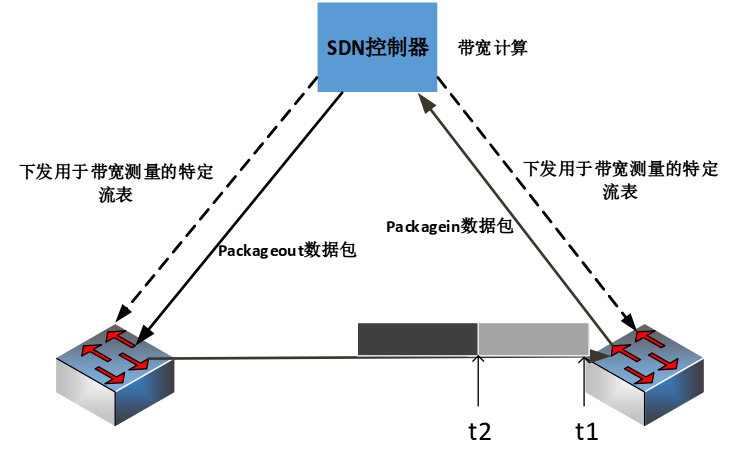
\includegraphics[width=0.6\textwidth]{logo/spaceband}
  \caption{链路可用带宽测量模型}
  \label{fig:spaceband}
\end{figure}

为了在数据包中存储到达目的交换机的时间,本文对OVS交换机进行源码变更,在匹配到特殊数据包(用于测量带宽的特定数据包,用特殊的IP地址标识)时,对数据包做改动,将数据包IPv6字段替换成当下时间,而后将数据包发送给控制器,控制器从数据报中解析出到达交换机的时间,即可得到背靠背数据包到达目的交换机的时间差,数据包的大小与时间差的比值,即为当前链路的可用带宽。而对于测量用的数据包,本文通过SDN控制器模拟一个满足需求的特定数据包下发给交换机,用于在交换机之间进行传输。

对于OVS的二次开发,主要涉及到对特定数据包的修改工作,即将数据包中的IPv6字段替换为当前的时间,具体如伪代码\ref{code-2}所示。由伪代码可以看出,本文对特定数据包的要求为源、目的IP均为0,由于该数据包由SDN控制器模拟产出,而且在实际的生活中是不存在的,所以不影响整个系统的运行。

\begin{algorithm}[!htb]
    \caption{OVS为数据包添加当下时间}
    \label{code-2}
    \begin{algorithmic}[1] %每行显示行号
        \Require 数据包,$packet$
        \Ensure 包含当前时间的数据报,$newpacket$
        \Function {modifyIPv6totime}{$packet$}
        	\State $srcip \gets packet.get('srcipv4')$
        	\State $dstip \gets packet.get('dstipv4')$
        	\If{$srcip==0$ \textbf{and} $dstip==0$}
        		\State $localtime \gets time.time$
        		\State $packet.update(ipv6, localtime)$
        	\EndIf
      		\State $newpacket \gets packet$
      		\State \Return{$newpacket$}
        \EndFunction
    \end{algorithmic}
\end{algorithm}

对于控制器端主要开发的功能包括,第一、模拟源、目的IP都为0的IP数据包。第二、为两个交换机下发用于测量带宽的流表。第三、对于控制器接收到的数据包,如果数据包满足源、目的IP都为0,则对数据包进行解析,获取时间差,计算当前链路的可用带宽。具体如伪代码\ref{code-3}所示。

\begin{algorithm}[!htb]
    \caption{SDN控制器测量可用带宽}
    \label{code-3}
    \begin{algorithmic}[1] %每行显示行号
        \Require 链路的源、目的交换机信息、数据包,$srcswitch,dstswitch,packets$
        \Ensure 当前链路的可用带宽,$bandwidth$
        \Function {add\_flow}{$srcswitch,dstswitch$}
        	\State $srcaction \gets [OFPActionOutput(2),OFPActionOutput(2)]$
        	\State $dstaction \gets [OFPPCONTROLLER]$
        	\State $macth \gets OFPMatch(src="0.0.0.0",dst="0.0.0.0")$
        	\State $addFlowMod(srcswitch,match,srcaction)$
        	\State $addFlowMod(dstswitch,match,dstaction)$
        \EndFunction
        \Function {simulatePacket}{$srcswitch$}
        	\State $pkt \gets packet.Packet()$
        	\State $pkt.update(ipv4(srcip="0.0.0.0",dstip="0.0.0.0"))$
        	\State $sendpacketout(pkt, srcswitch)$
        \EndFunction
         \Function {calculateBandwidth}{$packets$}
         	\State $starttime \gets packets[0].get(ipv6)$
         	\State $endtime \gets packets[1].get(ipv6)$
         	\State $bandwidth \gets (packets[0].size()/(endtime-starttime))$
         	\State \Return{$bandwidth$}
        \EndFunction
    \end{algorithmic}
\end{algorithm}
\subsection{已用带宽测量}
对于已用带宽的测量,本文基于数据包统计的方案实现。由第二章中的表\ref{table:flow}可以看出,流表中具有计数器字段,计数器用于统计流表被匹配的次数,以及匹配的数据包的大小。本文基于此,提出了基于计数器的已用带宽测量,通过统计某段时间内,从交换机某端口发出/接受的数据包数,取平均值进行已用带宽的测量工作,具体实现如伪代码\ref{code-4}所示。

\begin{algorithm}[!htb]
    \caption{SDN控制器测量已用带宽}
    \label{code-4}
    \begin{algorithmic}[1] %每行显示行号
        \Require 链路的源、目的交换机信息,端口号,$srcswitch,srcport,dstswitch,dstport$
        \Ensure 当前链路的已用带宽,$bandwidth$
        \Function {get\_counters}{$srcswitch,srcport, dstswitch,dstport$}
        	\State $inputBytes \gets getCounters(srcswitch, inport=srcport)$
        	\State $outputBytes \gets getCounters(srcswitch, outport=srcport)$
        	\State $allBytes \gets (inputBytes+outputBytes)$
        	\State \Return{$allBytes$}
        \EndFunction
        \Function {calculateBandwidth}{$srcswitch,srcport, dstswitch,dstport$}
        	\State $bytes1 \gets GET_{-}COUNTERS(srcswitch,srcport, dstswitch,dstport)$
        	\State $time.sleep(sometime)$
        	\State $bytes2 \gets getcounters(srcswitch,srcport, dstswitch,dstport)$
        	\State $bandwidth \gets ((bytes2-bytes1)/sometime)$
         	\State \Return{$bandwidth$}
        \EndFunction
    \end{algorithmic}
\end{algorithm}
\subsection{时延测量}
时延的测量,本研究采用最基本的基于三角模型的测量方法。即控制器与两台交换机组成最小的测量单元,分别测出控制器到交换机的时延以及三边的总时延,做差值即为链路的时延。模型如图\ref{fig:delay}所示,图中链路的时延即为t3-(t1+t2)/2。

\begin{figure}[!htb]
  \centering
  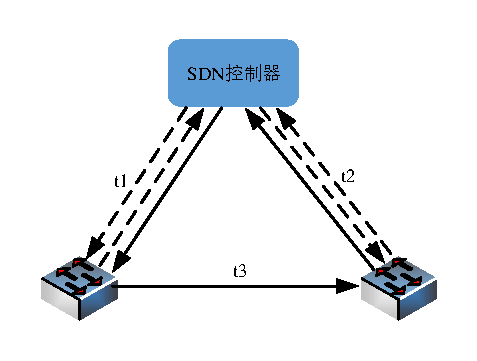
\includegraphics[width=0.6\textwidth]{logo/delay}
  \caption{链路时延测量模型}
  \label{fig:delay}
\end{figure}

具体实现如伪代码\ref{code-5}所示。主要包含流表下发、数据包模拟、时延计算模块,首先计算数据包从控制器到交换机的时延,需要为交换机下发流表,匹配到特定数据包以后,返回给控制器,而后控制器模拟出符合该匹配规则的数据包,发送给交换机,记录当前的时间,数据包到达交换机后,匹配上特定流表,数据包返还给控制器,至此控制器根究当前时间,利用时间差求解出控制器到交换机的时延。同理可以得到控制器->源交换机->目的交换机->控制器的时延,利用前面的公式即可得到链路的时延信息。

\begin{algorithm}[!htb]
    \caption{SDN控制器测量链路时延}
    \label{code-5}
    \begin{algorithmic}[1] %每行显示行号
        \Require 链路的源、目的交换机信息,端口号,$srcswitch,srcport,dstswitch,dstport$
        \Ensure 当前链路的时延,$delay$
        \Function {add\_flow}{$srcswitch,dstswitch,srcaction,dstaction$}
        	\State $macth \gets OFPMatch(srcmac="00:00:00:00:00:00",dstmac="00:00:00:00:00:00")$
        	\State $addFlowMod(srcswitch,match,srcaction)$
        	\State $addFlowMod(dstswitch,match,dstaction)$
        \EndFunction
        \Function {simulatePacket}{$switch$}
        	\State $pkt \gets packet.Packet()$
        	\State $pkt.update(mac(src="00:00:00:00:00:00",dst="00:00:00:00:00:00"))$
        	\State $sendpacketout(pkt, switch)$
        \EndFunction
         \Function {calculateDelay}{$packets$}
         	\State $t1 \gets time(controller->srcswitch->controller)$
         	\State $t2 \gets time(controller->dstswitch->controller)$
         	\State $t3 \gets time(controller->srcswitch->dstswitch->controller)$
         	\State $delay \gets (t3-(t1+t2)/2)$
         	\State \Return{$delay$}
        \EndFunction
    \end{algorithmic}
\end{algorithm}

\subsection{定制化流表下发}
定制化流表的下发,主要是根据用户定制化的链路信息,进行流表的下发工作,从而实现数据传输路径的定制化,即租户可以根据当前拓扑的负载情况,选择一条最优的链路,通过定制化流表的下发,实现数据的高效传输。输入的数据为Json格式的链路信息。具体数据如下。

\begin{python} 
link = {
	'hosts':{
		'src':{
			'mac':'type:str'
		},
		'dst':{
			'mac':'type:str'
		}
	}, #链路两端的主机信息,包括源主机的mac地址,目的主机的mac地址
	'switches':[
		{
			'dpid':'type:str',
			'in_port':'type:int',
			'out_port':'type:int'
		}
	] #交换机列表集合,对于每一个交换机,主要包括交换机的ID号、输入端口、输出端口
}
\end{python}

具体实现如伪代码\ref{code-6}所示,针对用户发送的数据信息,分别对交换机下发定制化的流表。这里针对每个交换机,均要添加反向流表。从而实现主机的双向通信。

\begin{algorithm}[!htb]
    \caption{SDN定制化流表下发}
    \label{code-6}
    \begin{algorithmic}[1] %每行显示行号
        \Require 定制化链路信息,$link$
        \Function {add\_flow}{$switch,match,out_{-}port$}
        	\State $action \gets [OFPActionOutput(out_{-}port)]$
        	\State $addFlowMod(switch,match,action)$
        \EndFunction
        \Function {add\_customflow}{$link$}
        	\State $hosts \gets link['hosts']$
        	\State $switches \gets link['switches']$
        	\State $srcmac \gets hosts['src']['mac']$
        	\State $dstmac \gets hosts['dst']['mac']$
        	\For{$switch$ \textbf{in} $switches$}
        		\State $match1 \gets OFPMatch(srcmac=srcmac,in_{-}port=switch['in_{-}port'])$
        		\State $match2 \gets OFPMatch(srcmac=dstmac,in_{-}port=switch['out_{-}port'])$
            	\State $ADD_{-}FLOW(switch,match1,switch['out_{-}port'])$
            	\State $ADD_{-}FLOW(switch,match2,switch['in_{-}port'])$
            \EndFor        	
        \EndFunction
    \end{algorithmic}
\end{algorithm}

\section{GUI模块}
本模块主要实现前端可视化操作,为租户提供操作的便捷性,本文中基于力导向图,实现了拓扑图的自动布局。该模式下,会对全网的整个拓扑图进行自动定位,节点与节点之间的互斥力,保证了节点的不可重合性。与此同时,拓扑元素可以实现可拖拽功能和手动定位功能,极大地提高了用户体验性。对于拓扑展示,本文主要实现了SDN物理网络、SDN虚拟网络的拓扑展示,在各自的拓扑图基础上,实现相应功能的具体操作和展示。具体如下。

\subsection{物理网络显示图}
物理网络的拓扑显示如图\ref{fig:physicalnet}所示,黑色的交换机代表云平台内部的br-int网桥,蓝色交换机是用OVS模拟的物理服务器之间的交换机集群,由图可以看出,租户可以进行物理网络的初始化,力导向图可以对拓扑中的元素进行自动布局。在此基础上,租户可以进行全局网络可用带宽的测量,测量数据会在相应的链路之上进行显示。通过对链路的点击选取,在输入框输入租户自有控制器的IP地址,可以实现vSDN网络的创建,创建的虚拟网路由租户自己的控制器进行集中管控。除此之外,租户亦可以进行删除虚拟网络的操作。

\begin{figure}[!htb]
  \centering
  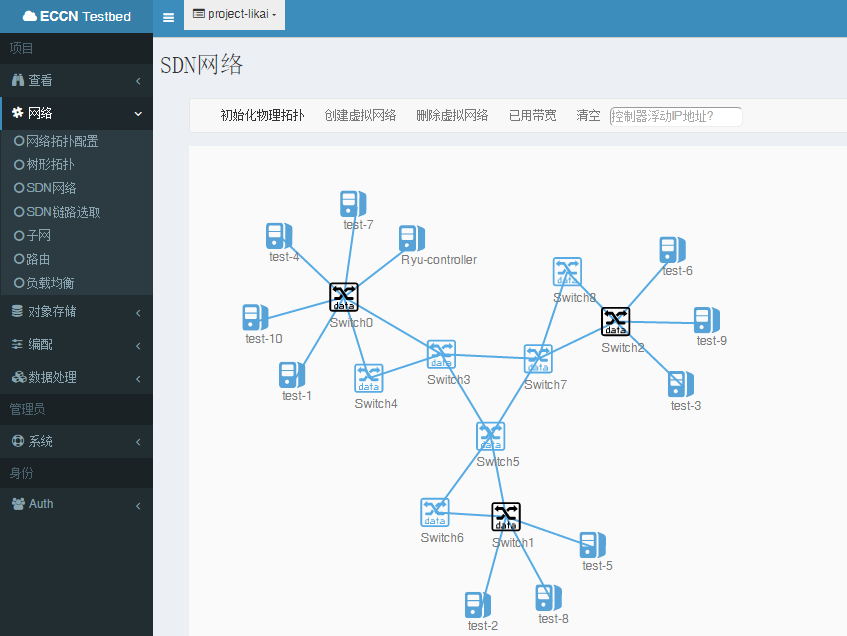
\includegraphics[width=0.8\textwidth]{logo/physicalnet.png}
  \caption{物理网络拓扑显示图}
  \label{fig:physicalnet}
\end{figure}

\subsection{虚拟网络显示图}
虚拟网络的拓扑显示图如图\ref{fig:virtualnet}所示,该界面主要是实现对租户虚拟网络的拓扑展示,由图中可以看出租户可以进行虚拟网络图的初始化,虚拟网络的删除,虚拟网络已用带宽、时延的显示,以及选路功能。带宽、时延的测量数据会在拓扑图相应链路上进行显示,对于选路功能,租户通过点击链路的方式进行数据传输链路的定制化,后台通过解析链路信息,下发定制化流表,实现特定数据传输路径的设置。

\begin{figure}[!htb]
  \centering
  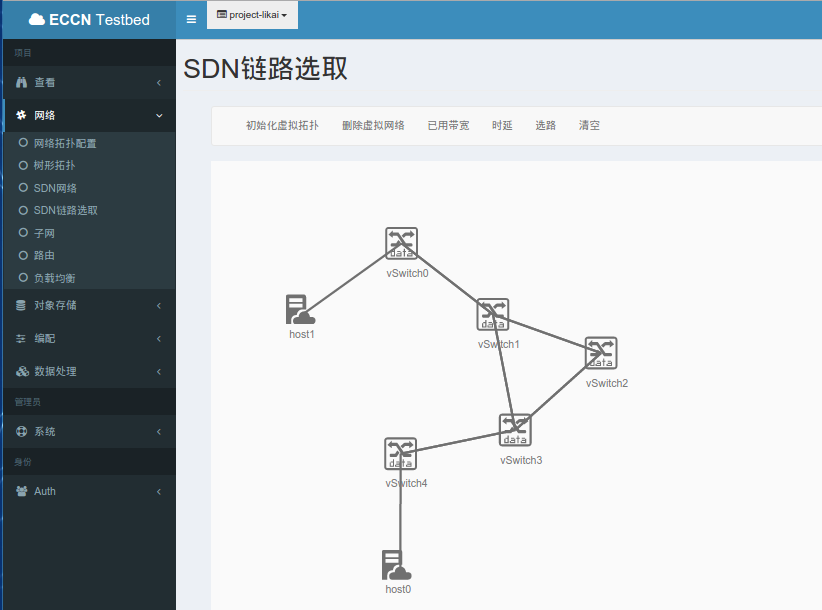
\includegraphics[width=0.8\textwidth]{logo/virtualnet.png}
  \caption{虚拟网络拓扑显示图}
  \label{fig:virtualnet}
\end{figure}

\section{本章小结}
本章主要对系统功能的具体实现做了详细的介绍。首先论文介绍了网络虚拟化模块,对虚拟化和去虚拟化的流程做了详细的解读,分别对PacketIn、PacketOut、FlowMod的虚拟化和去虚拟化的流程进行了讲解。针对虚拟网络的创建,在伪代码中做了详细介绍。通信模块主要介绍了基于RabbitMQ实现进程间通信的代码实现。对于控制器模块,本文对SDN模式下,可用带宽、已用带宽、时延定制化流表下发进行了详细的介绍。最后在GUI模块中,介绍了物理网络、虚拟网络拓扑图的前端显示,以及在相应模块上实现的不同功能。